\resourceheading{2}{Many Ways to Be a Good Classmate}{Autism inclusion, peer culture \& social-emotional learning}{Teachers, specialists \& families}{Module 1 taught Kit for Kids lesson and a documented Grade 2 technology routine}

\vspace{-0.5cm}
\toolsection{What This Resource Is}

Environmental access is only part of inclusion; peer culture can either preserve or undo it. This ten-minute peer-education lesson turns ``be kind'' into four observable actions: \textsc{invite, wait, ask, and respect}. It draws on the Organization for Autism Research (OAR) Kit for Kids, the \textit{What's Up with Nick?} booklet, and grade-banded friendship tips \citep{oar2026kit,oar2026nick,oar2026tips}. The lesson normalizes different ways of communicating, learning, moving, regulating, and participating. Students need language for helping without taking over, waiting without rushing, offering space without excluding, and accepting communication through speech, writing, pictures, AAC, gesture, movement, or silence. During camp, peer support sometimes looked similarly ordinary: continuing shared work, giving another person room, and keeping a route back into participation open rather than making that person's behavior the focus \citep{campEvidence2026}.

\toolsection{Ten-Minute Lesson Sequence}

\small
\renewcommand{\arraystretch}{1.15}
\setlength{\tabcolsep}{5pt}

\begin{tabularx}{\textwidth}{
>{\bfseries\RaggedRight\arraybackslash}p{0.75in}
>{\RaggedRight\arraybackslash}p{1.60in}
>{\RaggedRight\arraybackslash}X}

\rowcolor{PrimaryRed}
\color{white}Time &
\color{white}Move &
\color{white}Teacher Language and Student Action \\

0--2 min & Preview &
Show \textit{first/next/last}. ``Brains and bodies work in different ways. Good classmates help everyone participate without asking anyone to explain private information.'' \\

\rowcolor{SoftGray}
2--4 min & Teach &
Introduce the four actions below with one example and one nonexample each. \\

4--8 min & Practice &
Present one authentic classroom scenario. Pairs name a barrier, choose an action, and explain how it preserves choice. \\

\rowcolor{SoftGray}
8--10 min & Commit/close &
Students complete: ``One way I can support a classmate is...'' by speaking, writing, drawing, pointing, or passing and returning later. \\

\end{tabularx}

\normalsize

\toolsection{Four Peer Actions}

\setlength{\tabcolsep}{5pt}

\begin{tabularx}{\textwidth}{
>{\bfseries\color{DeepNavy}\RaggedRight\arraybackslash}p{0.72in}
>{\RaggedRight\arraybackslash}X
>{\RaggedRight\arraybackslash}X}

Invite &
Offer a role, seat, material, or turn without forcing a response. &
``Would you like to test, point, watch first, or choose another role?'' \\

\rowcolor{SoftGray}
Wait &
Leave processing time and keep the floor available. &
Count silently; do not repeat the question faster or answer for the person. \\

Ask &
Ask what support helps rather than guessing from a diagnosis or behavior. &
``Do you want help, more time, space, or a different way?'' Include ``something else.'' \\

\rowcolor{SoftGray}
Respect &
Protect communication tools, sensory needs, boundaries, breaks, privacy, and refusal. &
Do not grab a device, require eye contact, disclose a diagnosis, or make support conditional on compliance. \\

\end{tabularx}

\vfill

\begin{center}
\begin{tikzpicture}[
action/.style={draw=DeepNavy, rounded corners=2pt, minimum width=1.45in,
minimum height=0.60in, align=center, font=\scriptsize, inner sep=4pt},
next/.style={-{Latex[length=1.7mm]}, line width=0.7pt, draw=PrimaryRed}
]
\node[action, fill=SoftBlue] (invite) {\textbf{INVITE}\\offer a real route};
\node[action, fill=SoftGold, right=0.13in of invite] (wait) {\textbf{WAIT}\\keep the floor open};
\node[action, fill=SoftGreen, right=0.13in of wait] (ask) {\textbf{ASK}\\support, do not guess};
\node[action, fill=SoftRose, right=0.13in of ask] (respect) {\textbf{RESPECT}\\tools, boundaries, refusal};

\draw[next] (invite) -- (wait);
\draw[next] (wait) -- (ask);
\draw[next] (ask) -- (respect);

\node[font=\scriptsize\bfseries, text=DeepNavy,
below=0.09in of $(wait.south)!0.5!(ask.south)$]
{Choice stays with the learner};
\end{tikzpicture}
\end{center}

\newpage
\toolsection{Practice Scenario}

During a technology activity, one student has entered the program while several peers are still stuck. Another student is new to the routine. Ask: \textit{What barrier is present? What can a peer do without taking over? How can the person decline help?} Strong responses include showing one click, giving time to try, lowering voice volume, keeping the Chromebook in the learner's control, including the new student as part of the class, and accepting ``no thanks.''

\begin{center}
\colorbox{SoftGreen}{\parbox{0.93\textwidth}{\small
\textbf{Documented student evidence from the taught lesson:} One Grade 2 student proposed showing the next click without grabbing a classmate's Chromebook. Another said a new person should not be made to feel left out. These responses show students applying \textit{wait}, \textit{respect}, and \textit{invite} inside the actual technology routine.
}}
\end{center}

Use the same lesson before robotics, group building, recess transitions, digital publishing, or showcases. Revisit one action during the real routine; inclusion is learned through repeated practice, not one awareness event.

\reflectionbox{I taught this ten-minute lesson immediately before a partner-based Grade 2 coding and robotics routine. The strongest design move was locating support inside the activity rather than giving an abstract lecture: students had to decide how to help classmates enter a program without taking over and how to include a visitor in the classroom community \citep{placement2026robotics}. Ten minutes established shared language, but repeated practice is necessary before the four actions become a dependable peer norm. In Puzzle Plan terms, peer behavior becomes part of the access context; EQUITAS asks whether helping preserves the other student's authorship and right to decline.}

\adaptationbox{Ten minutes introduces shared language but cannot represent the full range of autistic experience. Pair OAR's educator material with autistic-authored perspectives when developmentally appropriate, adapt examples to age and culture, and monitor whether peers begin to police difference under the banner of helping. Adult redesign remains necessary; peer kindness cannot compensate for inaccessible schedules, noise, tools, or instruction.}

\begin{center}

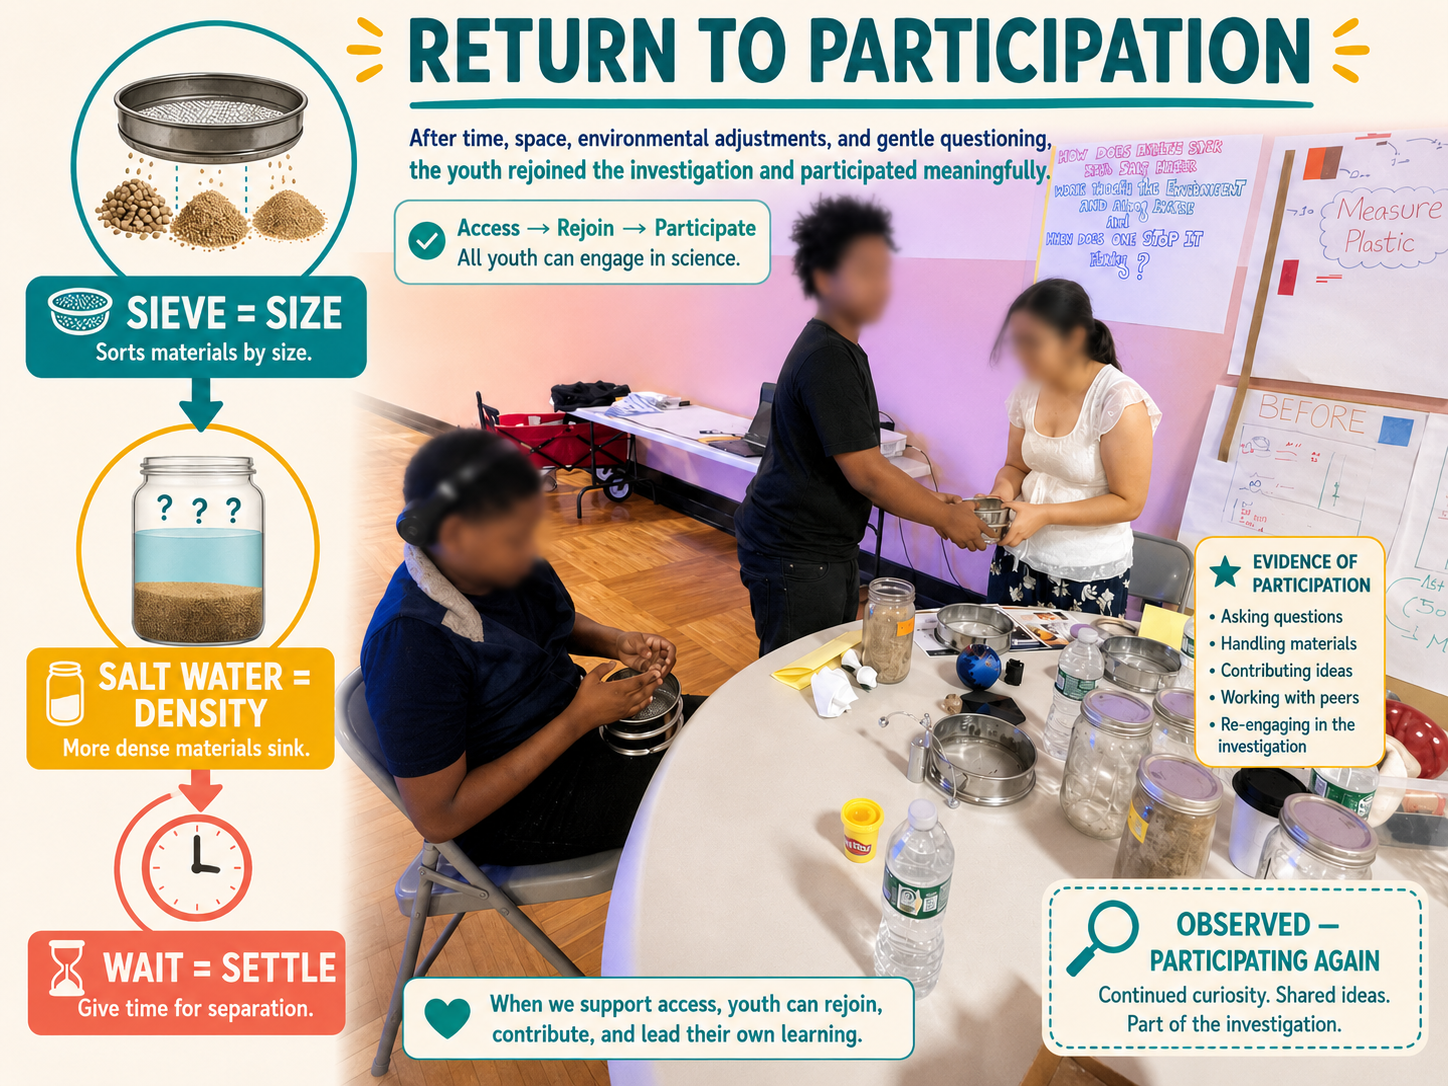
\includegraphics[
  width=0.75\textwidth,
  keepaspectratio
]{assets/artifact-previews/Return to Participation.png}

\parbox{0.90\textwidth}{\centering\scriptsize
\textbf{\color{DeepNavy}Peer Support in Practice.}
Camp practice illustrates the same peer norm: support can mean continuing shared work, giving a classmate room, and keeping a genuine route back into the investigation. The aim is not to manage another learner's behavior, but to preserve belonging without taking over.}

\end{center}

\sourcebox{\scriptsize OAR Kit for Kids \citep{oar2026kit}, \textit{What's Up with Nick?} \citep{oar2026nick}, and Friendship Tip Sheets \citep{oar2026tips}.}